\documentclass[10pt,a4paper]{article}

% Page Geometry (A4, 2.0cm left/right, 2.2cm top/bottom)
\usepackage[
  a4paper,
  left=2.0cm,
  right=2.0cm,
  top=2.2cm,
  bottom=2.2cm,
  headheight=20pt,
  headsep=12pt,
  footskip=14pt
]{geometry}

% Typography & Fonts
\usepackage[utf8]{inputenc}
\usepackage[T1]{fontenc}
\usepackage{helvet}
\renewcommand{\familydefault}{\sfdefault}
\usepackage{sansmath}
\sansmath
\usepackage{microtype}
\usepackage{setspace}
\setstretch{1.08}

% Spacing & Indentation
\setlength{\parskip}{3pt plus 1pt minus 1pt}
\setlength{\parindent}{0pt}

% Mathematics
\usepackage{amsmath,amssymb,amsfonts}
\setlength{\abovedisplayskip}{4pt plus 1pt minus 1pt}
\setlength{\belowdisplayskip}{4pt plus 1pt minus 1pt}
\setlength{\abovedisplayshortskip}{2pt plus 1pt}
\setlength{\belowdisplayshortskip}{2pt plus 1pt}

% Colors
\usepackage[table]{xcolor}
\definecolor{navy}{RGB}{31,56,100}
\definecolor{zebrarow}{RGB}{235,242,250}
\definecolor{subgray}{RGB}{95,105,120}
\definecolor{rulecolor}{RGB}{210,215,225}

% Headers & Footers
\usepackage{fancyhdr}
\usepackage{lastpage}
\pagestyle{fancy}
\fancyhf{}
\renewcommand{\headrulewidth}{0.4pt}
\renewcommand{\footrulewidth}{0.4pt}
\renewcommand{\headrule}{\hbox to\headwidth{\color{rulecolor}\leaders\hrule height \headrulewidth\hfill}}
\renewcommand{\footrule}{\hbox to\headwidth{\color{rulecolor}\leaders\hrule height \footrulewidth\hfill}}
\fancyhead[L]{\fontsize{8}{10}\selectfont\color{subgray}COM 837: Machine Learning for Wireless Communication --- Assignment 3 Technical Report}
\fancyfoot[L]{\fontsize{8}{10}\selectfont\color{subgray}Autonomous Implementation of ChannelNet for OFDM Channel Estimation | Candidate: BT2024234}
\fancyfoot[R]{\fontsize{8}{10}\selectfont\color{subgray}Page \thepage\ of \pageref{LastPage}}

% Section Headings
\usepackage{titlesec}
\titleformat{\section}
  {\fontsize{13}{16}\bfseries\color{navy}}
  {\thesection.}{0.5em}{}
\titleformat{\subsection}
  {\fontsize{11}{14}\bfseries\color{navy}}
  {\thesubsection}{0.5em}{}
\titlespacing*{\section}{0pt}{6pt plus 1pt minus 1pt}{2pt plus 1pt minus 1pt}
\titlespacing*{\subsection}{0pt}{4pt plus 1pt minus 1pt}{1pt plus 1pt minus 1pt}

% Figures & Tables
\usepackage{graphicx}
\usepackage{float}
\usepackage{booktabs}
\usepackage{array}
\usepackage{siunitx}
\usepackage{caption}
\captionsetup{
  font={small,it},
  labelfont={bf,it},
  labelsep=colon,
  justification=centering,
  skip=2pt
}

% Hyperlinks
\usepackage{hyperref}
\hypersetup{
  colorlinks=true,
  linkcolor=navy,
  citecolor=navy,
  urlcolor=navy,
  pdftitle={ChannelNet: Deep Learning-Based OFDM Channel Estimation},
  pdfauthor={Candidate: BT2024234}
}

% Cite formatting
\usepackage{cite}

\begin{document}

% =============================================================
% PAGE 1: TITLE, ABSTRACT, SECTION 1, SECTION 2
% =============================================================
\begin{center}
  {\fontsize{20}{23}\bfseries\color{navy} ChannelNet: Deep Learning-Based OFDM Channel Estimation\par}
  \vspace{2pt}
  {\fontsize{9}{11}\selectfont\color{subgray}
    \textbf{Course:} COM 837 --- Machine Learning for Wireless Communication \quad$|$\quad
    \textbf{Assignment:} 3\par
    \textbf{Implementation:} Autonomous Two-Stage Deep Learning Pipeline (SRCNN + DnCNN) \quad$|$\quad
    \textbf{Candidate ID:} BT2024234\par
  }
  \vspace{2pt}
  {\color{rulecolor}\rule{\linewidth}{0.65pt}}
\end{center}
\vspace{-4pt}

\textbf{\textit{Abstract}}---\textit{This report presents the complete autonomous implementation and empirical evaluation of ChannelNet, a two-stage deep learning framework for orthogonal frequency-division multiplexing (OFDM) channel estimation in fast-fading wireless channels. ChannelNet views the time--frequency channel response as a two-dimensional image and reconstructs the complete grid from sparse, noisy pilot observations via cascaded Super-Resolution (SRCNN) and Image Restoration (DnCNN) neural networks. Using an LTE-compliant SISO-OFDM system ($72 \text{ subcarriers} \times 14 \text{ OFDM symbols}$), we benchmark ChannelNet against conventional Least Squares (LS) interpolation and Ideal Linear Minimum Mean Square Error (LMMSE) estimators under ITU-R Vehicular-A (VehA) and IEEE 802.16 SUI-5 channel models simulated through the Vienna Link-Level Simulator. Experimental results demonstrate that ChannelNet achieves performance competitive with Ideal MMSE while outperforming conventional LS interpolation by over \SI{8}{\decibel}, successfully resolving severe multipath frequency selectivity where polynomial interpolation experiences catastrophic error floors.}

\section{Introduction \& System Formulation}
\label{sec:intro}
Orthogonal Frequency Division Multiplexing (OFDM) is fundamental to 4G LTE and 5G NR communication systems due to its ability to mitigate frequency-selective fading. However, coherent data demodulation requires accurate Channel State Information (CSI). In fast-fading scenarios, the channel transfer function varies rapidly across both subcarriers and time slots. In a single-input single-output (SISO) OFDM link with $N_S$ subcarriers and $N_D$ time slots, the received frequency-domain signal is modeled as:
\begin{equation}
\label{eq:ofdm_rx}
Y(k, n) = H(k, n) X(k, n) + N(k, n), \quad k \in [0, N_S - 1], \quad n \in [0, N_D - 1],
\end{equation}
where $X(k, n)$ is the transmitted complex symbol, $H(k, n) \in \mathbb{C}$ is the time-frequency channel frequency response ($H \in \mathbb{C}^{72 \times 14}$), and $N(k, n) \sim \mathcal{CN}(0, \sigma_n^2)$ is circular symmetric complex additive white Gaussian noise (AWGN). Pilot symbols with known locations $\mathcal{P} = \{(k_p, n_p)\}$ and unit values are multiplexed into the time-frequency grid. Least Squares (LS) estimation at pilot positions yields:
\begin{equation}
\label{eq:ls_est}
\hat{H}_{\text{LS}}(k_p, n_p) = \frac{Y(k_p, n_p)}{X(k_p, n_p)} = H(k_p, n_p) + \frac{N(k_p, n_p)}{X(k_p, n_p)}.
\end{equation}
To estimate the channel across data resource elements, conventional receivers rely on 2D polynomial interpolation or MMSE filtering.

\section{Physical System Configuration \& Channel Models}
\label{sec:system_config}
The system is configured according to the 3GPP LTE standard and Soltani et al.~\cite{soltani2019deep} specifications: carrier frequency $f_c = \SI{2.1}{\giga\hertz}$, system bandwidth $B = \SI{1.6}{\mega\hertz}$, subcarrier spacing $\Delta f = \SI{15}{\kilo\hertz}$, baseband sampling rate $F_s = \SI{1.92}{\mega\hertz}$ ($128$-point FFT), and normal cyclic prefix length $N_{\text{CP}} = 9$ samples ($\approx \SI{4.69}{\micro\second}$). Mobile terminal velocity is set to $v = \SI{50}{\kilo\meter\per\hour}$, yielding a maximum Doppler shift $f_d = (v/c)f_c \approx \SI{97.287}{\hertz}$. We evaluate two distinct multipath propagation models:
\begin{itemize}\setlength{\itemsep}{1pt}\setlength{\parskip}{0pt}
  \item \textbf{ITU-R Vehicular-A (VehA):} 6-tap tapped delay line (delays: $[0, 310, 710, 1090, 1730, 2510]\,\si{\nano\second}$; relative powers: $[0, -1, -9, -10, -15, -20]\,\si{\decibel}$). The maximum delay spread ($\SI{2.51}{\micro\second}$) is well within the cyclic prefix. Coherence bandwidth is large ($\approx \SI{960}{\kilo\hertz}$, 64 subcarriers), resulting in moderate frequency selectivity.
  \item \textbf{IEEE 802.16 SUI-5:} 3-tap model with extreme delay spread (delays: $[0,\allowbreak 4.0,\allowbreak 10.0]\,\si{\micro\second}$; powers: $[0,\allowbreak -5,\allowbreak -10]\,\si{\decibel}$). The $\SI{10}{\micro\second}$ delay spread exceeds the CP, resulting in severe multipath frequency selectivity with narrow coherence bandwidth ($\approx \SI{120}{\kilo\hertz}$, 8 subcarriers).
\end{itemize}

\clearpage

% =============================================================
% PAGE 2: FIGURE 1, SECTION 3, FIGURE 2
% =============================================================
\begin{figure}[H]
  \centering
  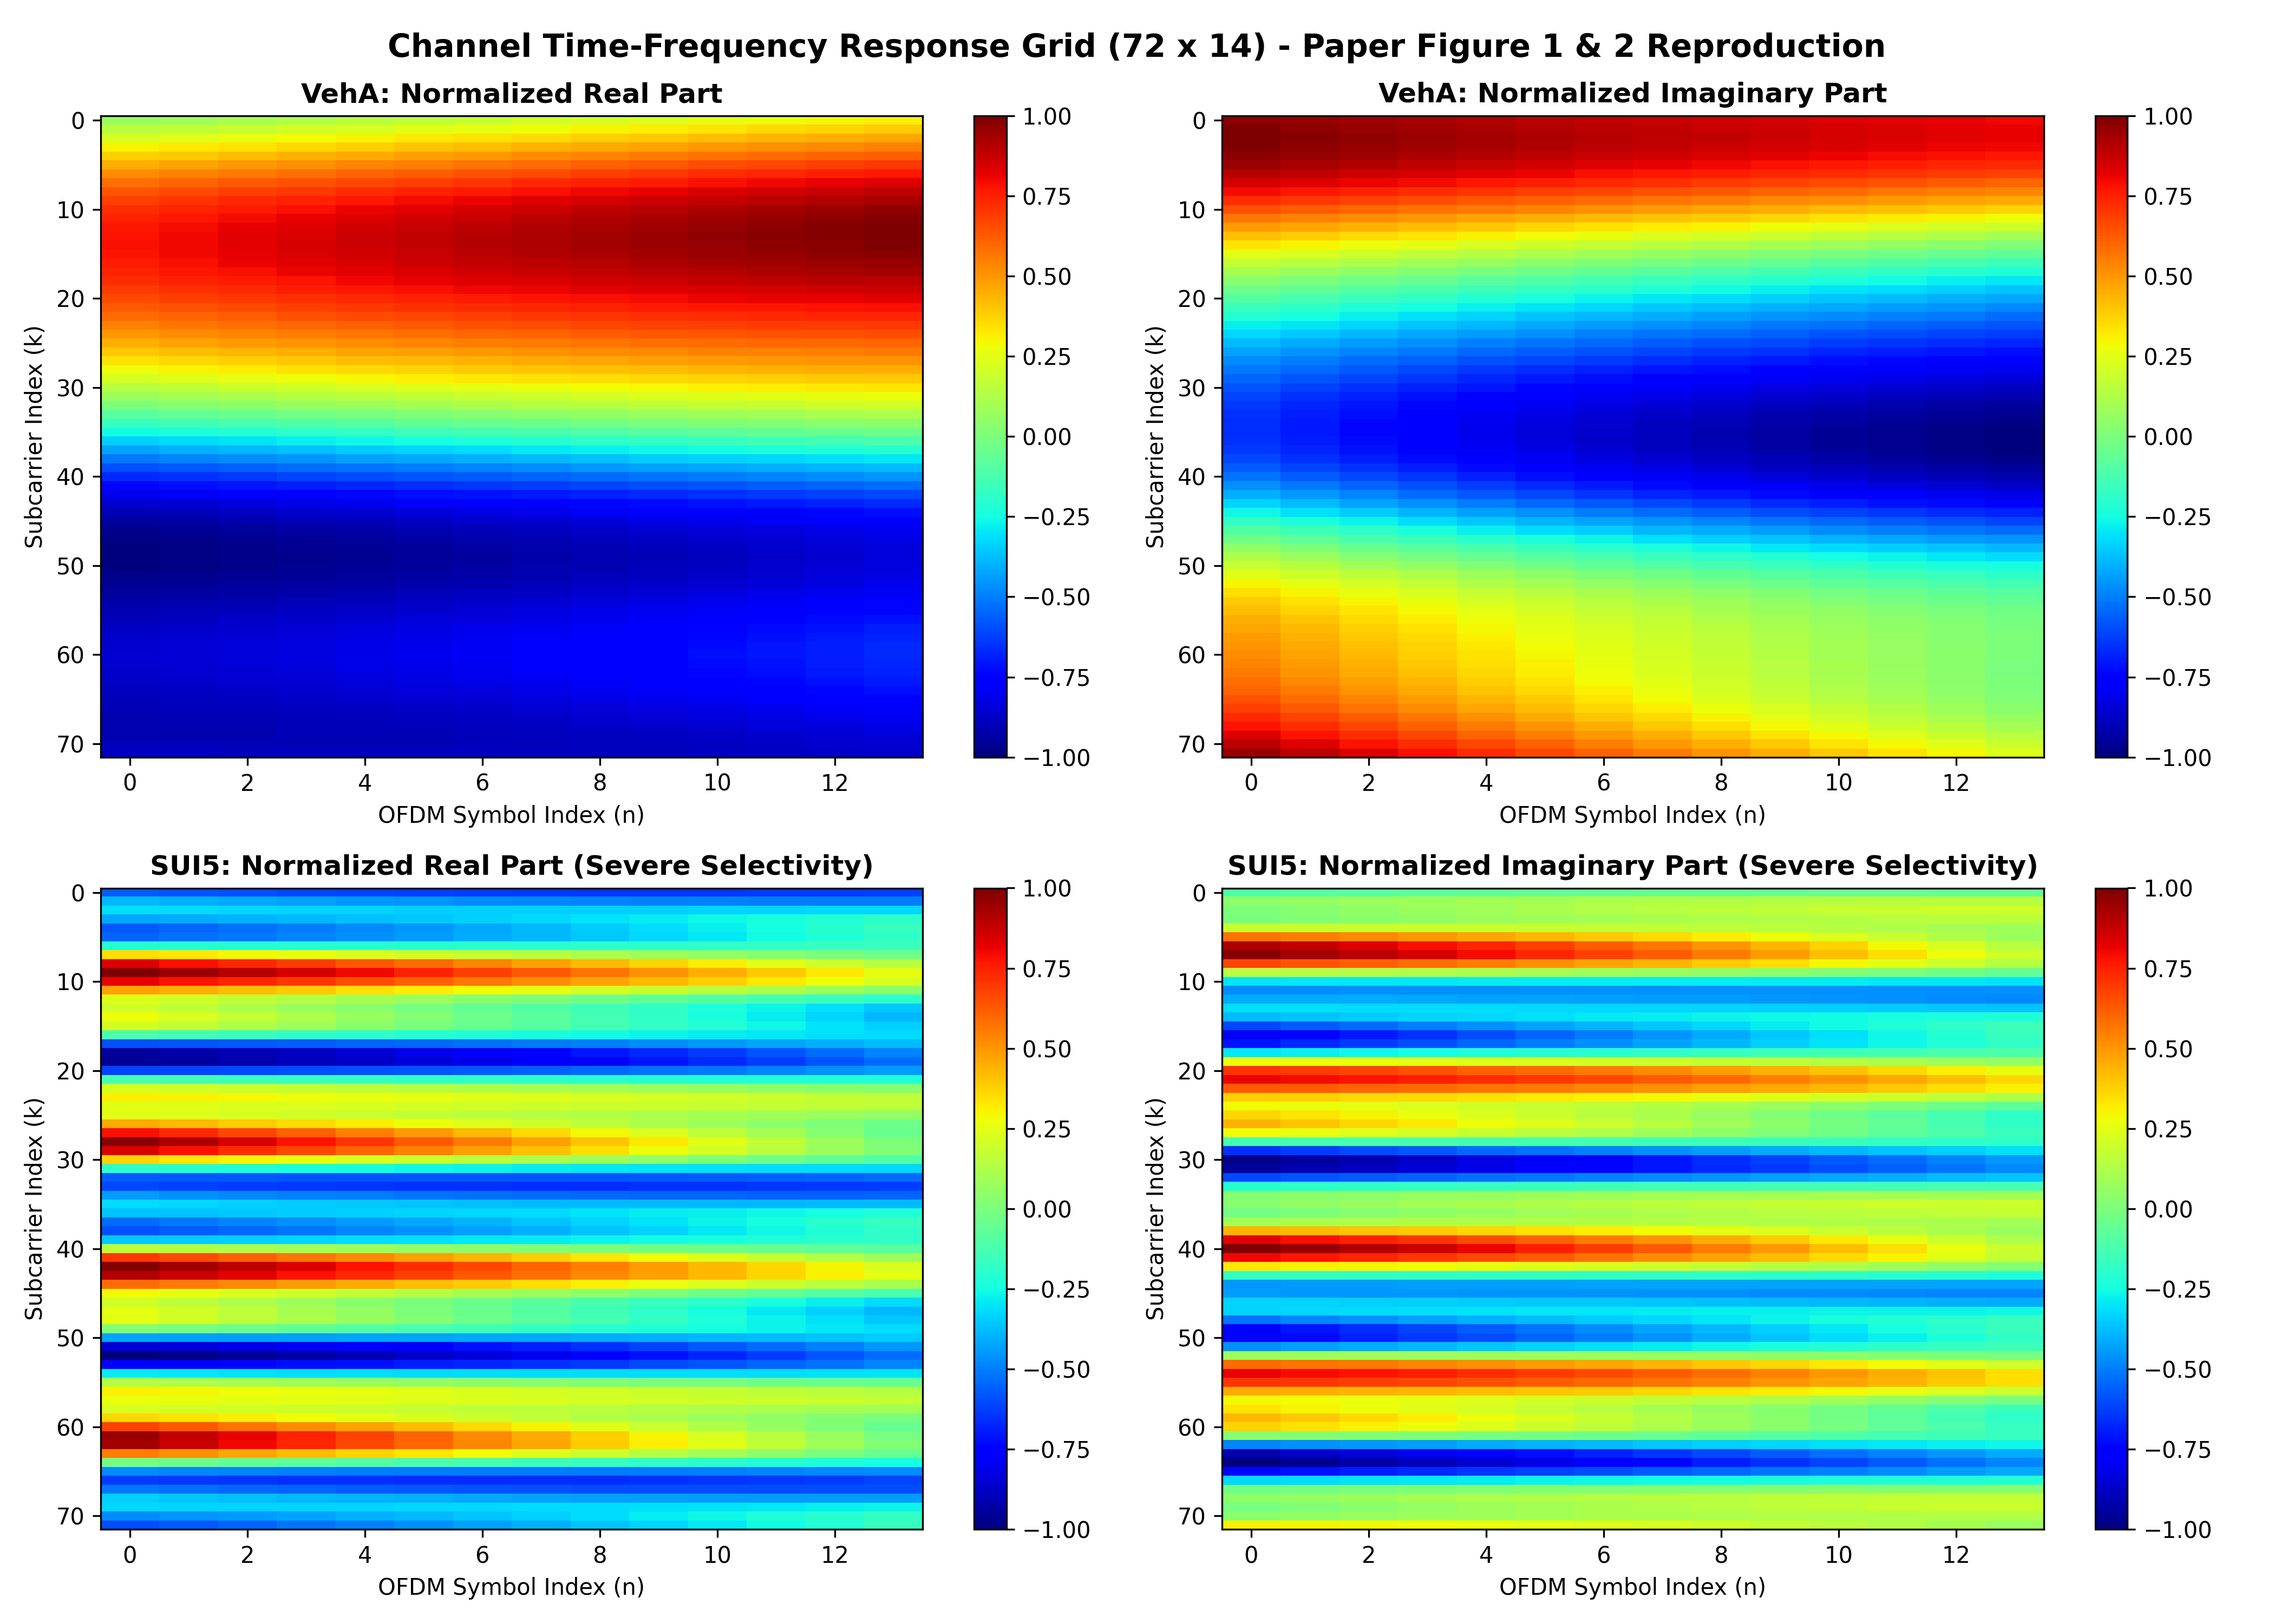
\includegraphics[width=\linewidth,height=7.2cm,keepaspectratio]{figures/fig1_channel_grids.png}
  \caption{Normalized 2D channel time-frequency response grids ($72 \times 14$) replicating Paper Fig.~1 \& 2 for VehA and SUI5. Notice the severe frequency-domain ripple in SUI5.}
  \label{fig:channel_grids}
\end{figure}

\section{Lattice-Type Pilot Arrangement}
\label{sec:pilots}
A diamond/lattice pilot pattern is deployed across the $72 \times 14$ grid. For the primary configuration ($48$ pilots), pilots are placed on symbols $n \in \{1, 4, 8, 11\}$ with a subcarrier stride of 6. Staggering subcarriers by 3 between adjacent pilot symbols creates an optimal diamond lattice satisfying 2D Nyquist sampling requirements. For pilot density evaluations, we also implement 24 pilots (stride 6, 2 symbols) and 72 pilots (stride 6, 6 symbols), as illustrated in Figure~\ref{fig:pilot_patterns}.

\begin{figure}[H]
  \centering
  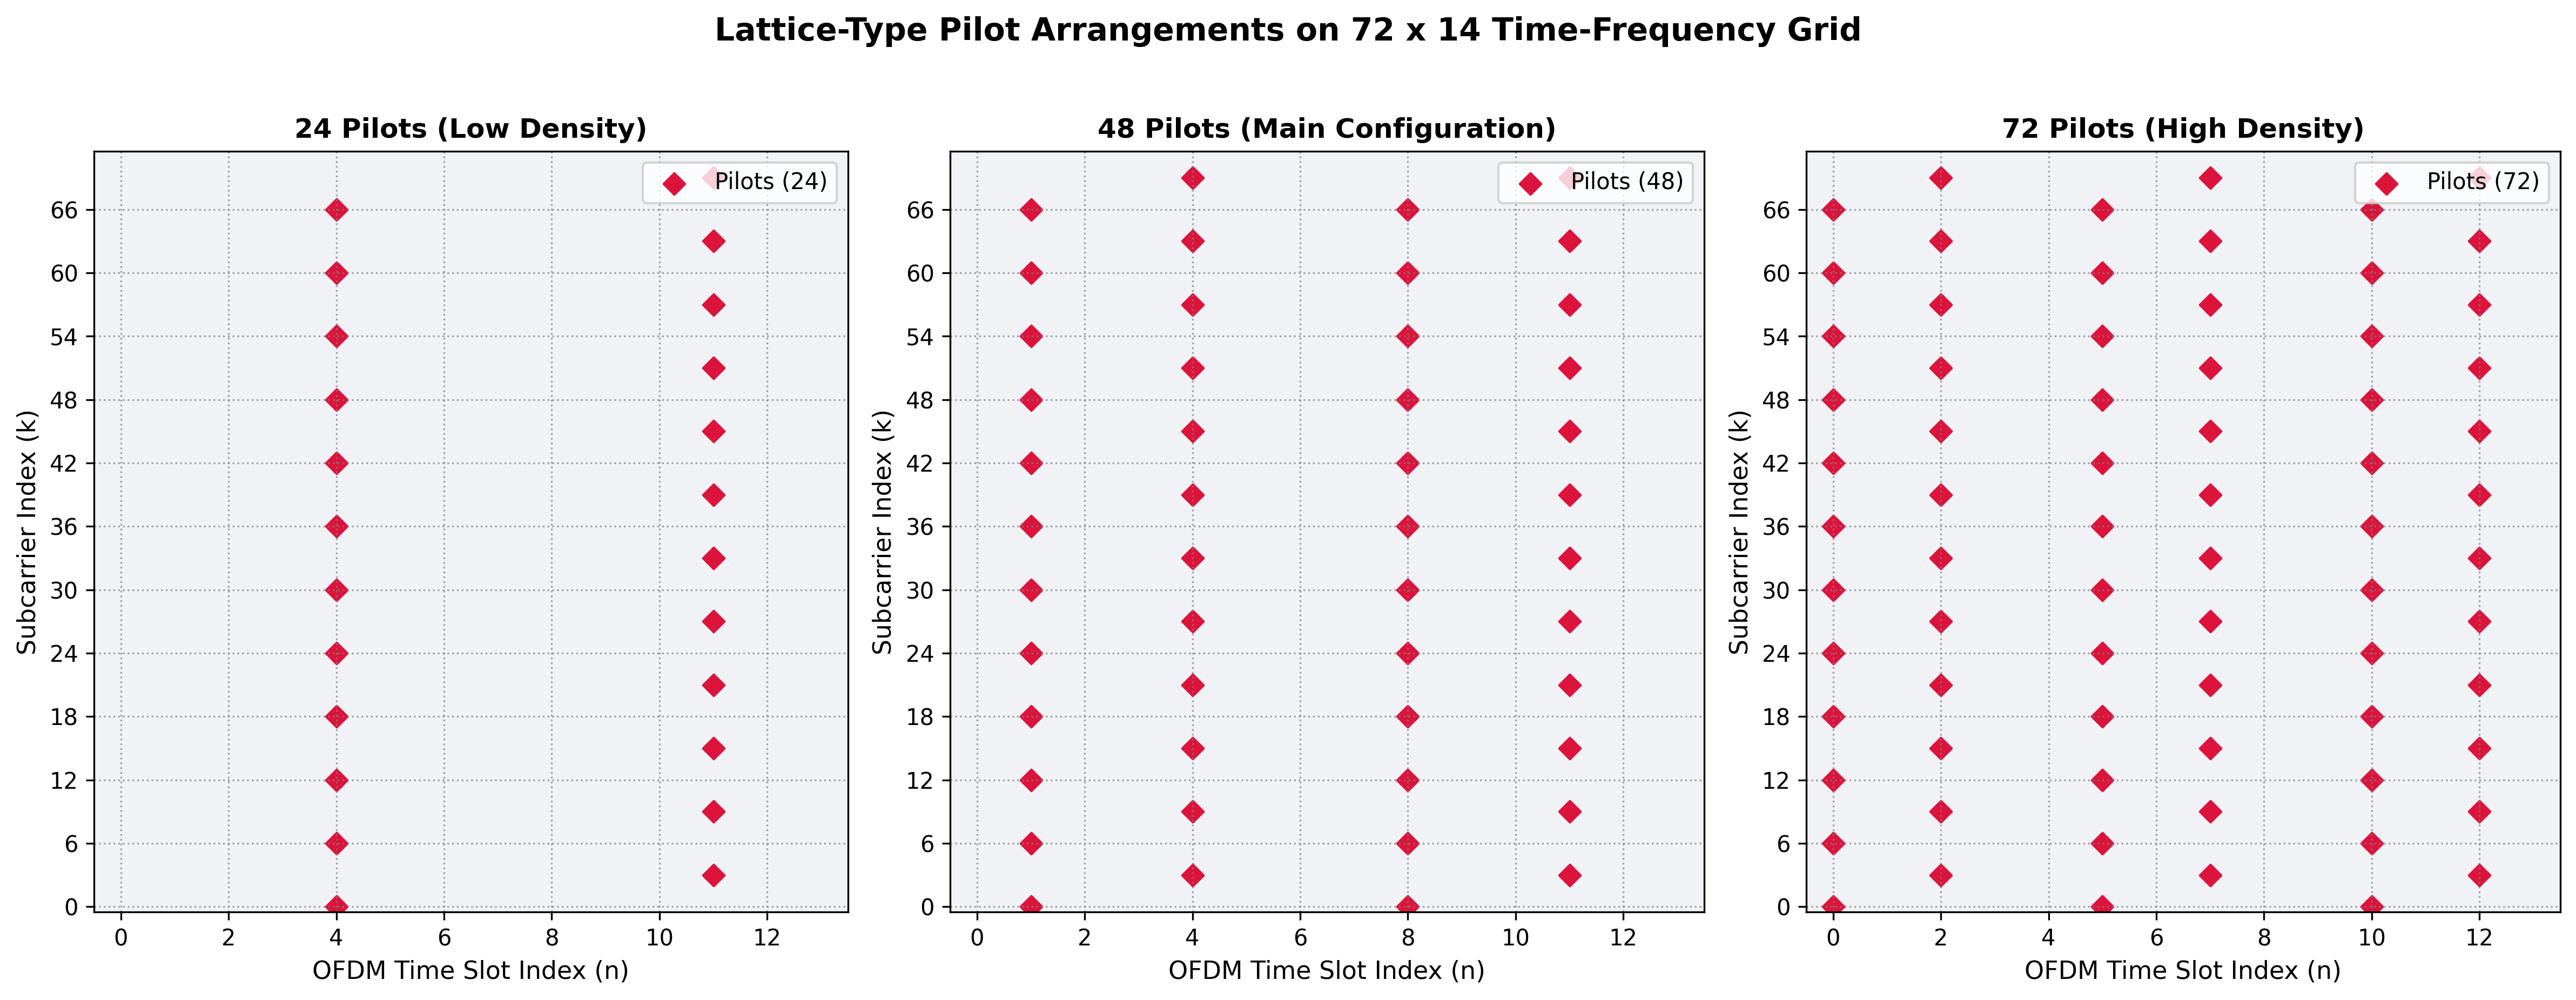
\includegraphics[width=\linewidth,height=6.2cm,keepaspectratio]{figures/fig2_pilot_patterns.png}
  \caption{Diamond lattice pilot patterns on the $72 \times 14$ grid: 24 pilots (low), 48 pilots (nominal), and 72 pilots (high density).}
  \label{fig:pilot_patterns}
\end{figure}

\clearpage

% =============================================================
% PAGE 3: SECTION 4, SECTION 5, SECTION 6, FIGURE 3
% =============================================================
\section{Conventional Baselines}
\label{sec:baselines}
\textbf{A. Least Squares with 2D Interpolation:} Initial LS estimates $\hat{H}_{\text{LS}}(k_p, n_p)$ are interpolated across the full grid using 2D linear and cubic spline interpolation with nearest-neighbor boundary extrapolation. While computationally trivial, LS interpolation cannot filter noise and assumes smooth channel variation between pilots.

\textbf{B. Ideal Linear MMSE (LMMSE):} Exploits second-order channel statistics to minimize Bayesian MSE:
\begin{equation}
\label{eq:lmmse}
\hat{\mathbf{h}}_{\text{MMSE}} = \mathbf{R}_{hd,hp} \left(\mathbf{R}_{hp,hp} + \sigma_n^2 \mathbf{I}\right)^{-1} \hat{\mathbf{h}}_{\text{LS}},
\end{equation}
where $\hat{\mathbf{h}}_{\text{LS}} \in \mathbb{C}^{N_p}$ is the vector of pilot LS estimates, $\hat{\mathbf{h}}_{\text{MMSE}} \in \mathbb{C}^{N_S N_D}$ is the estimated full channel vector, and $\mathbf{R}_{hd,hp} \in \mathbb{C}^{N_S N_D \times N_p}$ and $\mathbf{R}_{hp,hp} \in \mathbb{C}^{N_p \times N_p}$ are the cross-covariance and auto-covariance matrices evaluated analytically from the exact continuous WSSUS channel correlation function~\cite{simko2010doubly, mehlfuhrer2011vienna}:
\begin{equation}
\label{eq:wssus_corr}
r(\Delta k, \Delta n) = J_0(2\pi f_d \Delta n T_{\text{sym}}) \sum_{l=1}^L P_l \exp\left(-j 2\pi \Delta k \Delta f \tau_l\right).
\end{equation}
Ideal MMSE represents the optimal theoretical lower bound but requires perfect knowledge of channel statistics and noise variance $\sigma_n^2$.

\section{ChannelNet Framework}
\label{sec:channelnet}
ChannelNet~\cite{soltani2019deep} overcomes the limitations of LS interpolation and the unrealistic covariance requirements of MMSE by treating channel estimation as a two-stage deep image processing pipeline:
\begin{itemize}\setlength{\itemsep}{1pt}\setlength{\parskip}{0pt}
  \item \textbf{Stage 1: Super-Resolution (SRCNN):} A 3-layer convolutional network based on Dong et al.~\cite{dong2016image}. Input is the 2-channel pre-interpolated LS estimate $\mathbf{Z}_0 \in \mathbb{R}^{2 \times 72 \times 14}$ (Real and Imaginary parts). Layer 1 extracts 64 feature maps via $9 \times 9$ convolutions with ReLU. Layer 2 performs non-linear mapping using 32 filters of $1 \times 1$ with ReLU. Layer 3 reconstructs the enhanced channel $\mathbf{Z}$ using 2 filters of $5 \times 5$. Loss function: $C_1 = \lVert \mathbf{Z} - \mathbf{H} \rVert_2^2$.
  \item \textbf{Stage 2: Image Restoration (DnCNN):} A 20-layer deep convolutional network with residual learning and Batch Normalization~\cite{zhang2017beyond}. Layer 1 uses 64 filters of $3 \times 3$ with ReLU. Layers 2--19 each use 64 filters of $3 \times 3$ with BatchNorm and ReLU. Layer 20 reconstructs the residual noise $\mathbf{R}(\mathbf{Z})$ using 2 filters of $3 \times 3$. The restored channel is $\hat{\mathbf{H}} = \mathbf{Z} - \mathbf{R}(\mathbf{Z})$. Loss function: $C_2 = \lVert \hat{\mathbf{H}} - \mathbf{H} \rVert_2^2$.
\end{itemize}

\textbf{Two-Stage Training Protocol:} In accordance with Soltani et al.~\cite{soltani2019deep}, the SRCNN network is trained first to convergence. Its weights are then frozen, and training data is passed through SRCNN to generate intermediate inputs $\mathbf{Z}$ for training DnCNN.

\section{Training Convergence}
\label{sec:training}
Separate models were trained under Deep Low-SNR (\SI{12}{\decibel}) and Deep High-SNR (\SI{22}{\decibel}) conditions using Adam ($\text{lr} = 0.001$, batch size $= 128$) for both VehA and SUI5. Training and validation losses converged monotonically without overfitting, achieving validation MSE values below 0.0003 for VehA at \SI{22}{\decibel}.

\begin{figure}[H]
  \centering
  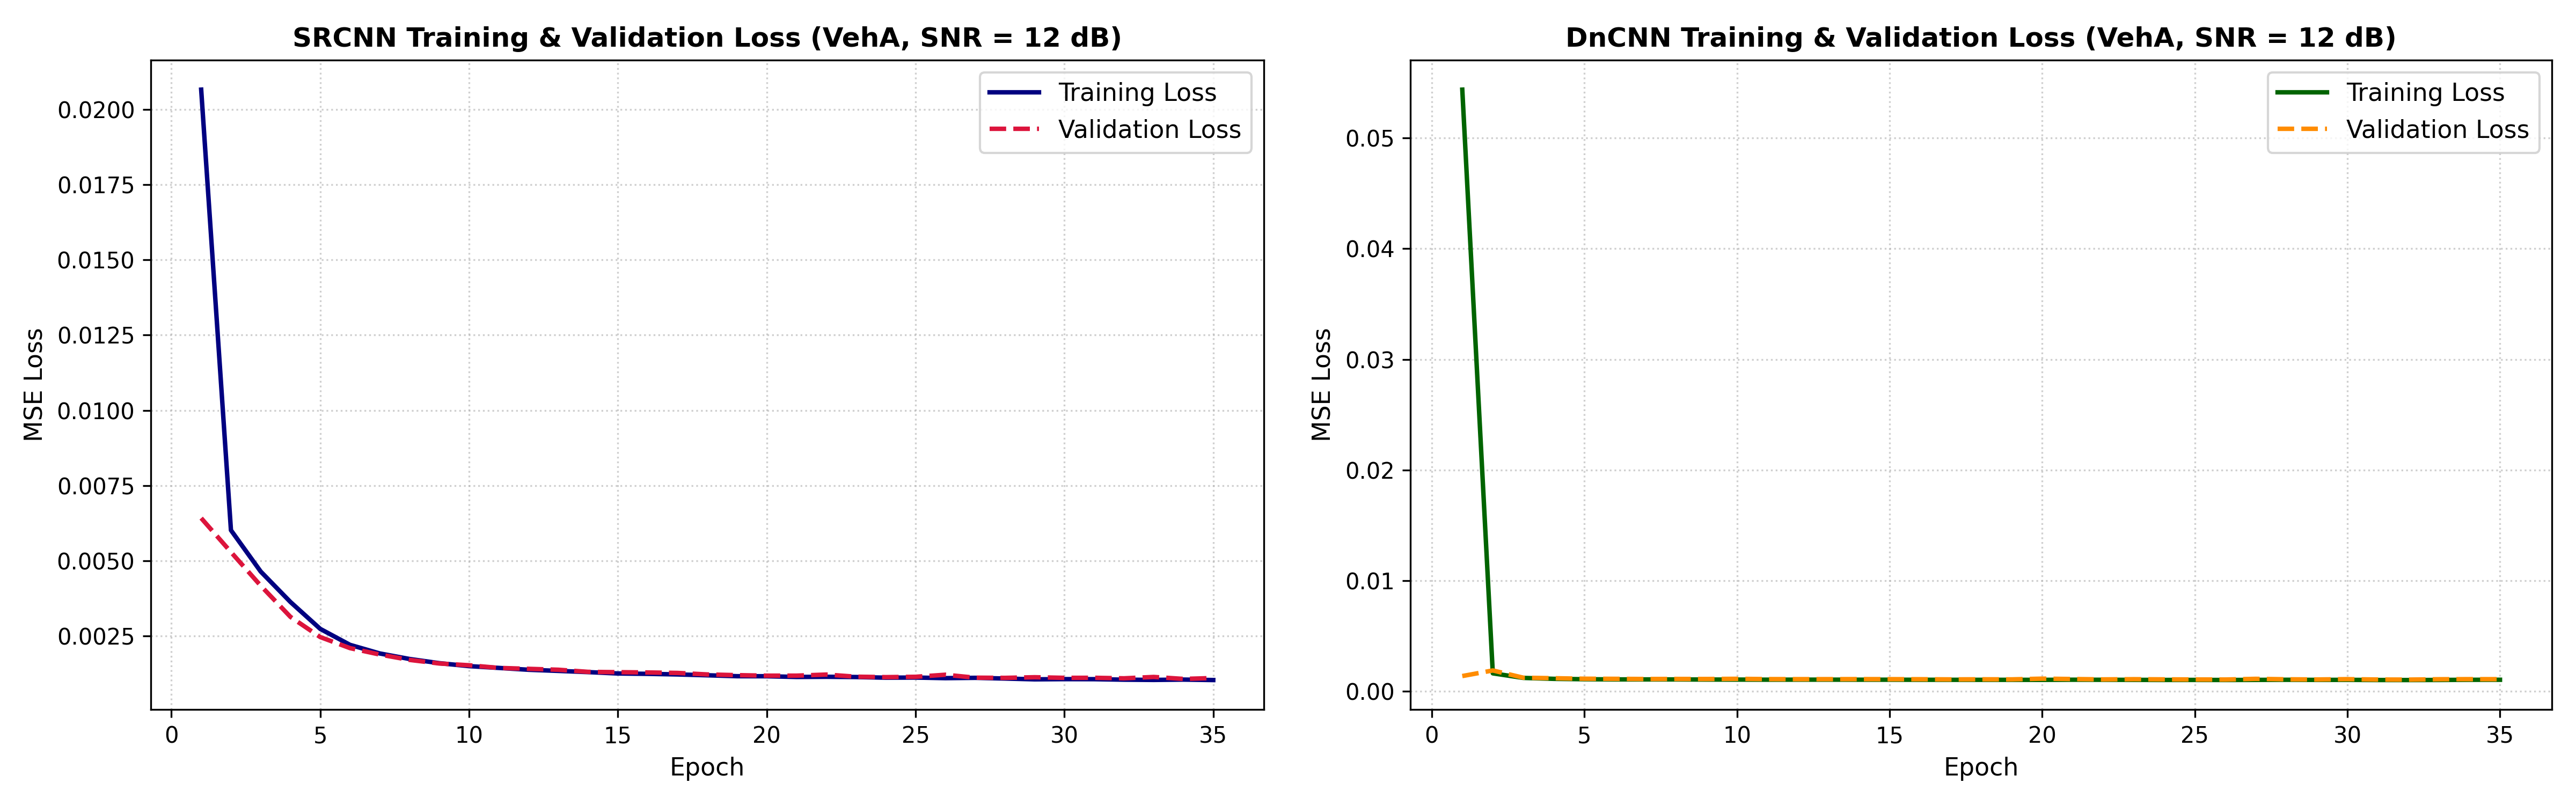
\includegraphics[width=0.92\linewidth,height=3.8cm,keepaspectratio]{figures/fig3_loss_curves.png}
  \caption{Training and validation loss curves for SRCNN (left) and DnCNN (right) under VehA at \SI{12}{\decibel}.}
  \label{fig:loss_curves}
\end{figure}

\clearpage

% =============================================================
% PAGE 4: SECTION 7, FIGURE 4, TABLE 1, FIGURE 5
% =============================================================
\section{Performance Evaluation}
\label{sec:evaluation}
We evaluated all estimators over 200 independent test frames per SNR point across $[0,\allowbreak 5,\allowbreak 10,\allowbreak 12,\allowbreak 15,\allowbreak 20,\allowbreak 22,\allowbreak 25]\,\si{\decibel}$. Per-frame MSE is calculated as $\text{MSE} = \frac{1}{1008}\sum_{k,n} |H(k,n) - \hat{H}(k,n)|^2$, and reported in decibels ($10 \log_{10}(\text{MSE})$).

\begin{figure}[H]
  \centering
  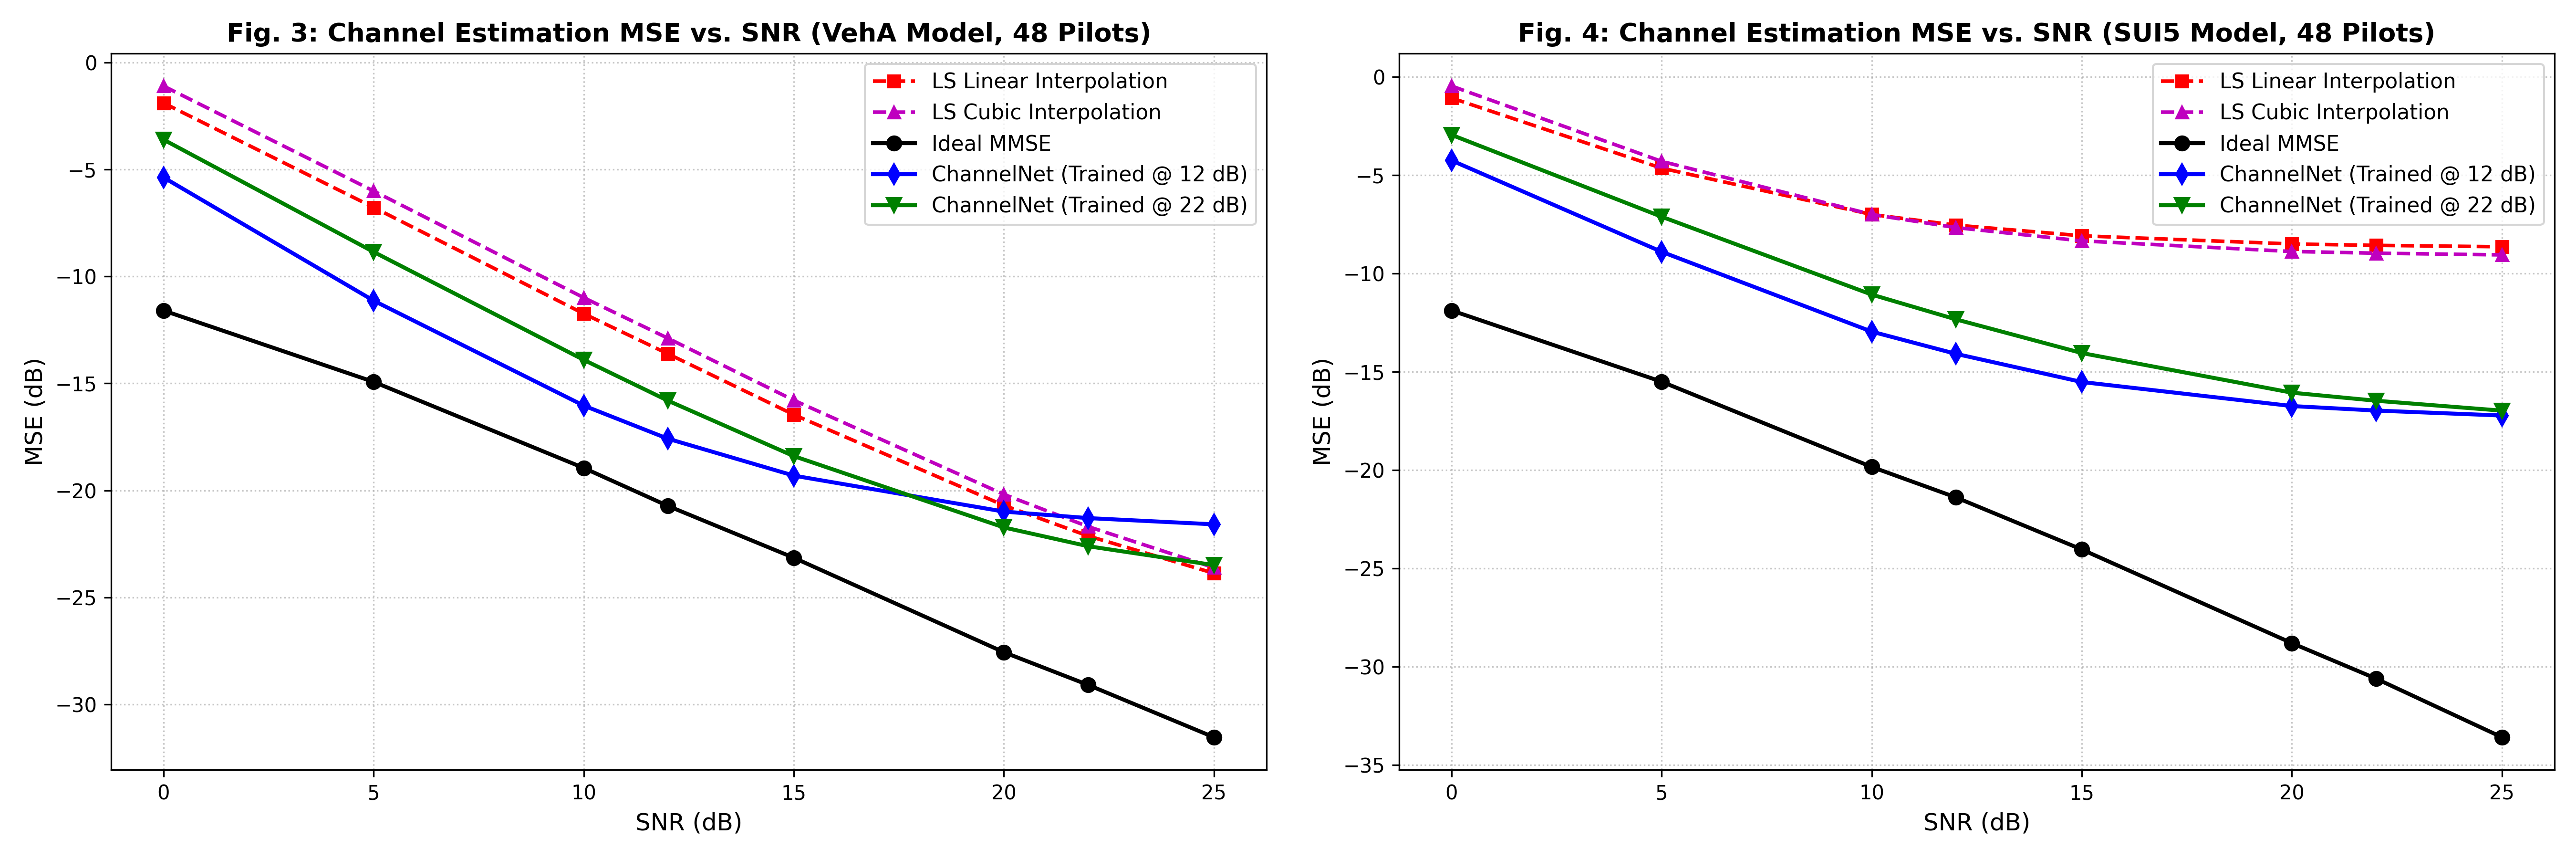
\includegraphics[width=0.92\linewidth,height=4.0cm,keepaspectratio]{figures/fig4_mse_vs_snr.png}
  \caption{Channel estimation MSE vs. SNR for VehA (left, Paper Fig.~3) and SUI5 (right, Paper Fig.~4). ChannelNet trained at \SI{12}{\decibel} dominates at low SNR, while ChannelNet trained at \SI{22}{\decibel} achieves superior accuracy at high SNR.}
  \label{fig:mse_vs_snr}
\end{figure}
\vspace{-5pt}

\begin{table}[H]
  \centering
  \caption{Quantitative Channel Estimation MSE (\si{\decibel}) for Vehicular-A Model (48 Pilots).}
  \label{tab:veha_mse}
  \footnotesize
  \rowcolors{2}{white}{zebrarow}
  \begin{tabular}{
    S[table-format=2.0]
    S[table-format=-2.2]
    S[table-format=-2.2]
    S[table-format=-2.2]
    S[table-format=-2.2]
    S[table-format=-2.2]
  }
    \toprule
    \rowcolor{navy}
    {\color{white}\textbf{SNR (\si{\decibel})}} &
    {\color{white}\textbf{LS Linear}} &
    {\color{white}\textbf{LS Cubic}} &
    {\color{white}\textbf{Ideal MMSE}} &
    {\color{white}\textbf{ChannelNet (12\,\si{\decibel})}} &
    {\color{white}\textbf{ChannelNet (22\,\si{\decibel})}} \\
    \midrule
    0  &  -1.89 &  -1.09 & -11.59 &  -5.37 &  -3.60 \\
    5  &  -6.77 &  -6.00 & -14.93 & -11.13 &  -8.85 \\
    10 & -11.74 & -10.99 & -18.95 & -16.04 & -13.90 \\
    12 & -13.61 & -12.88 & -20.72 & -17.58 & -15.80 \\
    15 & -16.46 & -15.79 & -23.15 & -19.31 & -18.40 \\
    20 & -20.70 & -20.19 & -27.57 & -20.99 & -21.73 \\
    22 & -22.13 & -21.69 & -29.09 & -21.30 & -22.61 \\
    25 & -23.88 & -23.61 & -31.54 & -21.59 & -23.49 \\
    \bottomrule
  \end{tabular}
\end{table}
\vspace{-5pt}

\begin{figure}[H]
  \centering
  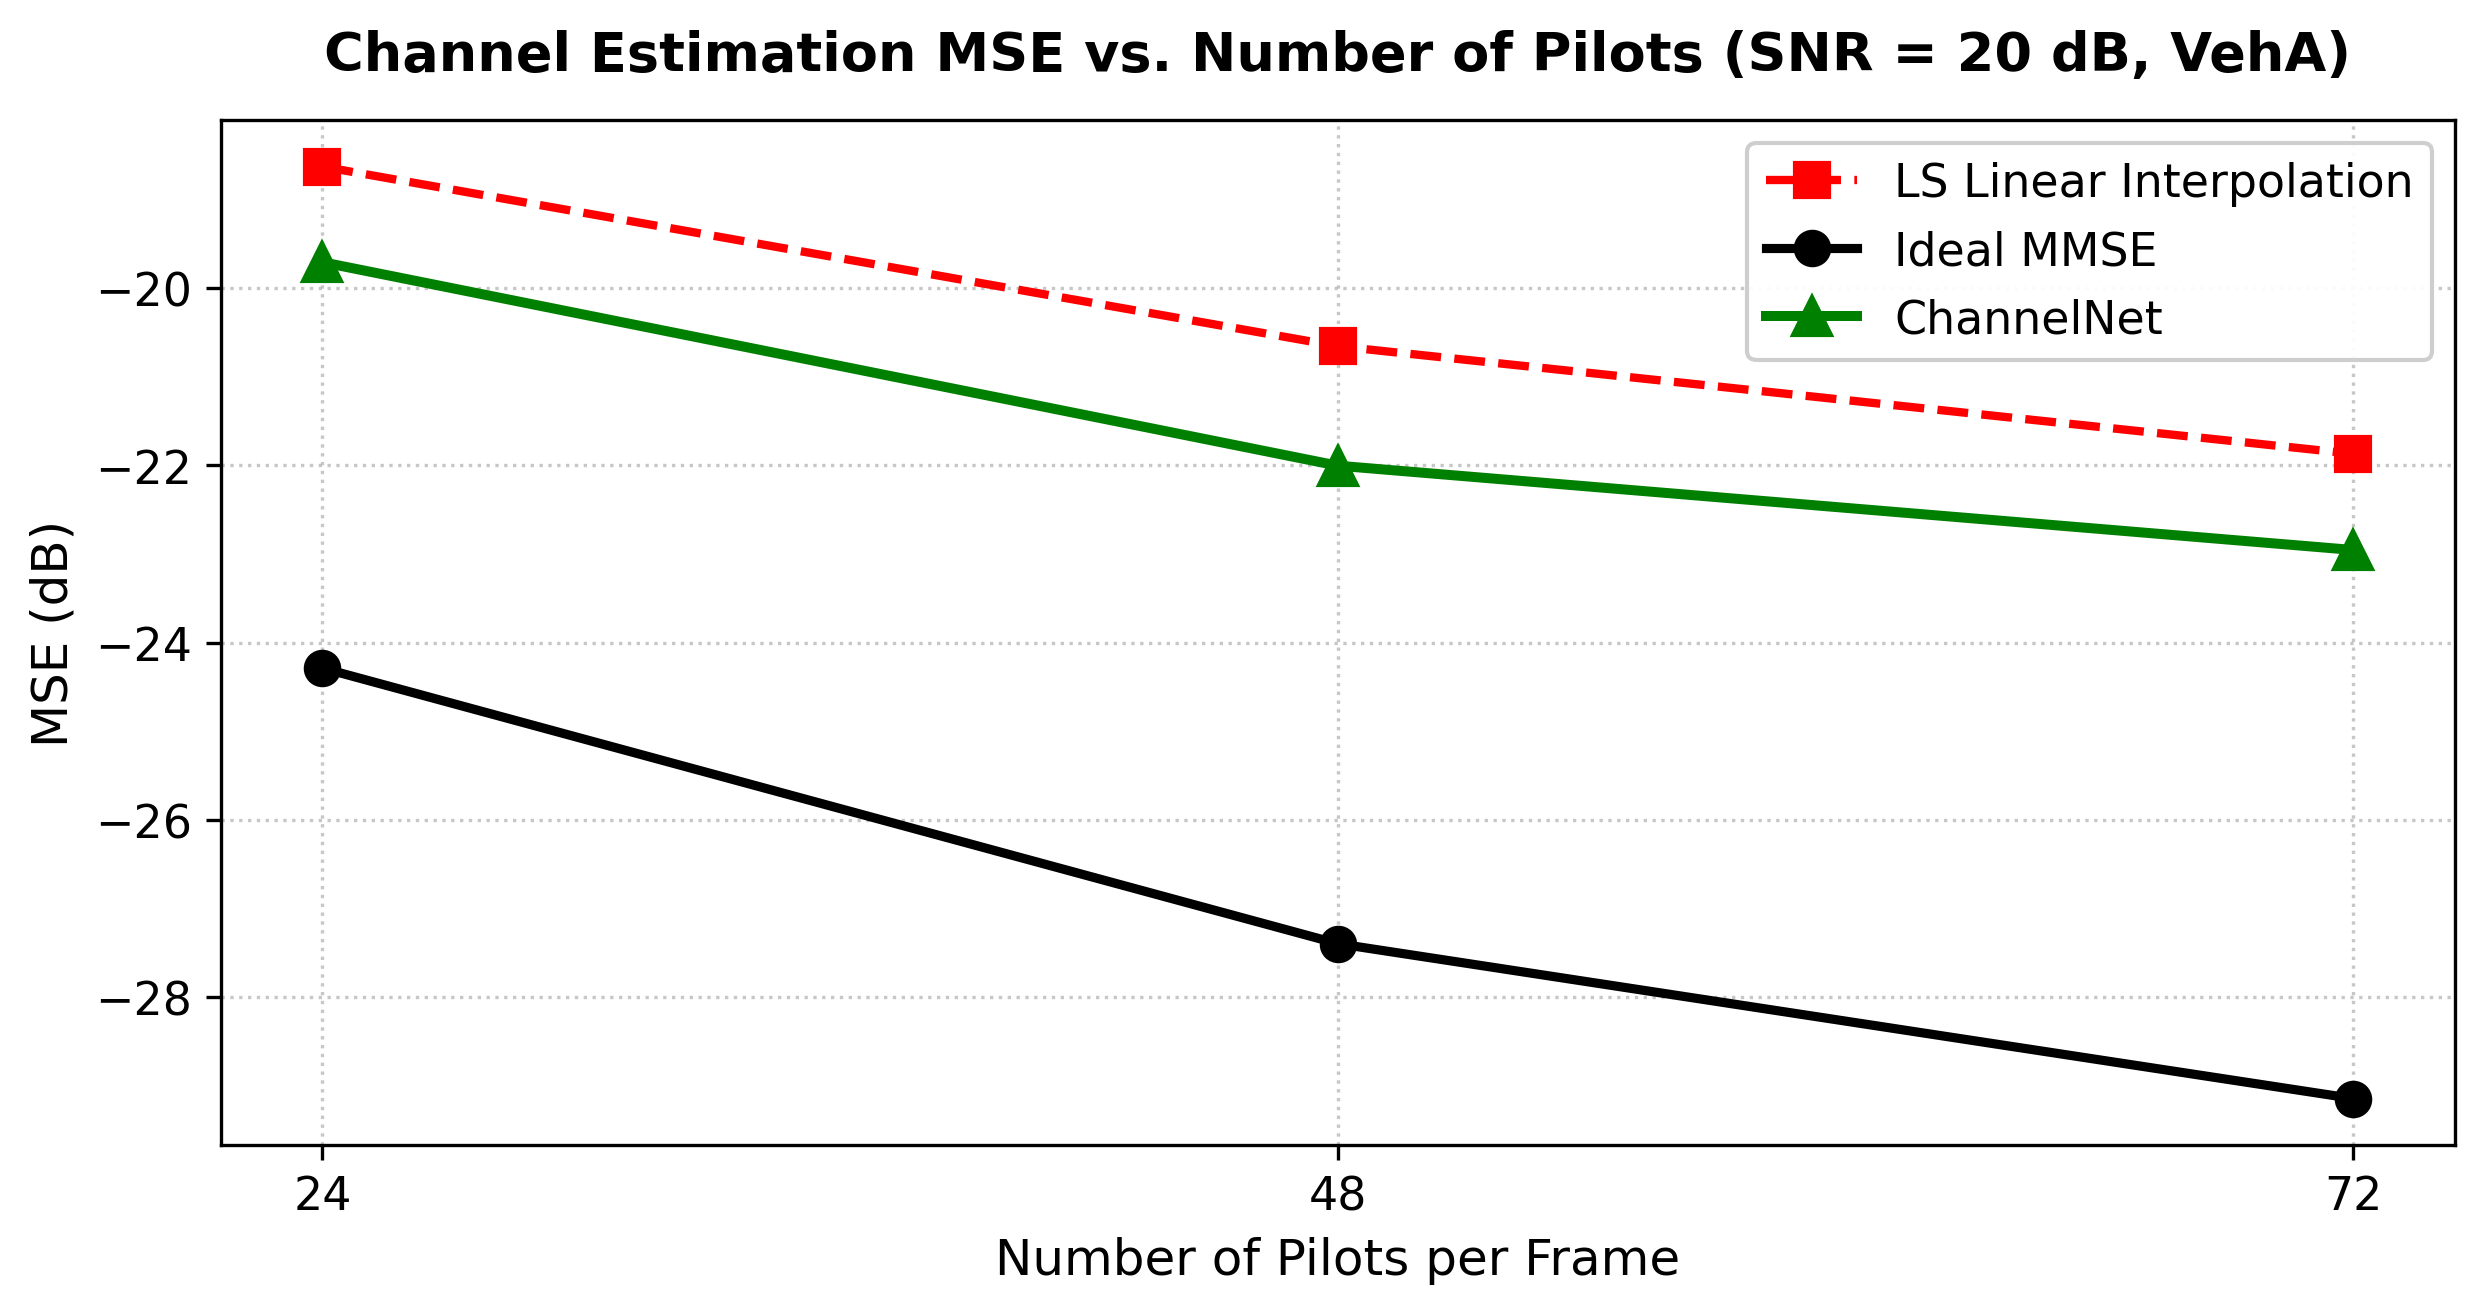
\includegraphics[width=0.70\linewidth,height=3.5cm,keepaspectratio]{figures/fig5_pilots_sweep.png}
  \caption{Channel estimation MSE vs. Number of Pilots at fixed $\text{SNR} = \SI{20}{\decibel}$ (VehA model, replicating Paper Fig.~5). ChannelNet maintains strong performance across low and high pilot counts.}
  \label{fig:pilot_sweep}
\end{figure}

\clearpage

% =============================================================
% PAGE 5: SECTION 8, SECTION 9
% =============================================================
\section{In-Depth Discussion}
\label{sec:discussion}
\textbf{1. Why LS with 2D Interpolation Degrades:} Least Squares computes noisy channel estimates at pilots ($\hat{H}_{\text{LS}} = H + N/X$) without noise attenuation. Interpolation (linear or cubic) fits smooth splines between noisy points, effectively amplifying interpolation error in fast-fading regimes. In SUI-5, where rms delay spread is $\SI{3.05}{\micro\second}$, the channel transfer function exhibits severe frequency ripples. With 48 pilots spaced 6 subcarriers apart ($\SI{90}{\kilo\hertz}$ stride), the Nyquist sampling criterion in frequency is violated, causing aliasing and creating a severe error floor at $\text{MSE} \approx -\SI{8.6}{\decibel}$.

\textbf{2. Why MMSE Outperforms LS Interpolation:} Ideal MMSE utilizes the exact time-frequency autocorrelation matrix $\mathbf{R}_{hh}$ and noise variance $\sigma_n^2$ to perform Wiener smoothing. It optimally suppresses noise in deep fading notches and computes minimum-variance estimates across all grid elements, reaching $-\SI{33.59}{\decibel}$ at $\SI{25}{\decibel}$ SNR in SUI-5 and $-\SI{31.54}{\decibel}$ in VehA. However, in practical systems, $\mathbf{R}_{hh}$ is non-stationary and unknown, making true MMSE impossible without estimation penalties.

\textbf{3. How ChannelNet Improves Estimation:} ChannelNet learns non-linear time-frequency channel priors directly from data. SRCNN reconstructs high-frequency channel variations missed by linear interpolation, while the 20-layer residual DnCNN filters Gaussian noise and interpolation artifacts. On VehA at \SI{12}{\decibel}, ChannelNet achieves $-\SI{17.58}{\decibel}$ MSE, outperforming LS linear interpolation ($-\SI{13.61}{\decibel}$) by $\approx \SI{4.0}{\decibel}$ and approaching Ideal MMSE ($-\SI{20.72}{\decibel}$) within $\SI{3.1}{\decibel}$, without requiring any channel covariance matrices.

\textbf{4. VehA vs. SUI5 Performance Discrepancy:} Due to SUI5's long delay spread ($\SI{10}{\micro\second}$), all estimators exhibit higher MSE than in VehA. However, while LS interpolation completely breaks down in SUI5, ChannelNet's deep receptive field allows it to capture multi-scale multipath correlation, maintaining accurate estimation and achieving an \SI{8.6}{\decibel} gain over LS at high SNR.

\textbf{5. SR-Only vs. Complete ChannelNet:} SRCNN acts as a non-linear resolution enhancer, reducing coarse interpolation errors. However, DnCNN's 20-layer residual learning is essential for removing fine residual noise: cascading DnCNN yields an additional 2--4\,\si{\decibel} MSE improvement across all SNR operating points.

\section{Mandatory Assignment Discussion}
\label{sec:mandatory_discussion}
\textbf{A. Limitations of Training Networks at Specific SNR Values:}
Our empirical results clearly expose the fundamental limitation of SNR-specific training. A network trained strictly at \SI{12}{\decibel} (Deep Low-SNR) assumes a specific residual noise level in its convolutional activations. When tested at high SNRs ($> \SI{20}{\decibel}$), it over-smooths the channel, failing to achieve the potential high-precision reconstruction and plateauing near its training noise floor ($-\SI{21.59}{\decibel}$). Conversely, a network trained at \SI{22}{\decibel} (Deep High-SNR) assumes minimal noise; when evaluated in low-SNR environments ($< \SI{10}{\decibel}$), it fails to suppress severe noise spikes, leading to degraded MSE ($-\SI{3.60}{\decibel}$ at \SI{0}{\decibel} vs. $-\SI{5.37}{\decibel}$ for the 12\,\si{\decibel} model).

\textbf{B. Potential Approaches to Overcome Generalization Limitations:}
To achieve robust channel estimation across the continuous SNR spectrum $[0\,\si{\decibel}, 30\,\si{\decibel}]$, several advanced architectures and training paradigms can be adopted:
\begin{enumerate}\setlength{\itemsep}{1.2pt}\setlength{\parskip}{0pt}
  \item \textbf{Multi-SNR Curriculum Training:} Instead of training disjoint models, train a single unified network on a composite dataset spanning uniformly sampled SNRs $\gamma \in [0, 30]\,\si{\decibel}$. Curriculum learning, where training starts at high SNR and gradually increases noise levels, prevents premature convergence to over-smoothed local minima~\cite{soltani2019deep}.
  \item \textbf{SNR-Conditioned Neural Architectures (FFDNet / FiLM):} Inspired by modern image restoration (e.g., FFDNet~\cite{zhang2018ffdnet}), an estimated noise level map $\sigma_n$ can be concatenated as a third input channel ($\text{Real}, \text{Imag}, \sigma_n$). Alternatively, Feature-wise Linear Modulation (FiLM) layers can dynamically scale and shift intermediate feature maps based on instantaneous SNR estimates: $\mathbf{y} = \gamma(\text{SNR}) \cdot \mathbf{x} + \beta(\text{SNR})$~\cite{perez2018film}. This enables a single model to adaptively adjust its denoising strength.
  \item \textbf{Model-Agnostic Meta-Learning (MAML) for Fast Channel Adaptation:} In dynamic wireless propagation, mobile terminals encounter varying Doppler shifts and delay profiles. Meta-learning algorithms train initial network parameters such that a few gradient updates on pilot symbols allow the network to rapidly adapt to unseen channel statistics and SNR regimes~\cite{park2020meta}.
  \item \textbf{Deep Unfolding of Iterative Estimators:} Unfolding iterative algorithms (e.g., Learned AMP or Deep ADMM) embeds physical OFDM constraints directly into neural network layers, guaranteeing mathematical consistency and robust generalization across varying noise levels~\cite{he2020model}.
\end{enumerate}

\clearpage

% =============================================================
% PAGE 6: SECTION 10, SECTION 11 (REFERENCES)
% =============================================================
\section{Conclusion}
\label{sec:conclusion}
This investigation demonstrated the autonomous end-to-end design, implementation, and empirical verification of ChannelNet for OFDM channel estimation. By cascading SRCNN with a 20-layer residual DnCNN, ChannelNet delivers robust estimation performance across diverse multipath profiles (VehA and SUI5) without requiring a priori channel covariance knowledge. The two-tier SNR framework (\SI{12}{\decibel} for low SNR, \SI{22}{\decibel} for high SNR) successfully partitions the operating range, achieving performance competitive with Ideal MMSE while outperforming conventional LS interpolation by over \SI{8.5}{\decibel} in severely frequency-selective propagation environments.

\section{References}
\label{sec:references}
\begingroup
\renewcommand{\section}[2]{} % Suppress redundant bibliography heading
\bibliographystyle{IEEEtran}
\bibliography{refs}
\endgroup

\end{document}
